\section{RQ3 -- Potential SSC Risks Imposed by LLM}
\label{sec:rq3}

\par As shown in Figure~\ref{fig:llmrisk},
 we summarized possible vulnerabilities  of an LLM, which
 may posit attack surfaces to the Software Supply Chain,
 across its lifecycle --
\textit{training \& tuning} stage, \textit{inference} stage,
and \textit{agent} stage.  This section then
delves into how these vulnerabilities turn against
Software Supply Chain security.

\begin{figure}
  % \documentclass{standalone}
% \usepackage{tikz}
% \usepackage{multirow}
% \usetikzlibrary{shapes.geometric}
% \usetikzlibrary{decorations.pathreplacing,calligraphy}
% \usetikzlibrary{positioning}
% \usetikzlibrary{arrows.meta}
% \begin{document}

\begin{tikzpicture}[
  every node/.style={fill=white},
  base/.style={rectangle, rounded corners, draw=blue!60, fill=blue!5, very thick, minimum size=2.5cm},
  sys/.style={rectangle, rounded corners, draw=green!60, fill=green!5, very thick, minimum size=2.5cm},
  vuln/.style={rectangle, rounded corners, draw=red!60, fill=red!5, very thick, minimum size=2.5cm},
]


\node[base] (tt) {
\begin{tabular}{cc}
  \multicolumn{2}{c}{\textbf{Training \& Tuning}} \\
  \begin{tikzpicture}[
  vuln/.style={rectangle, rounded corners, draw=red!60, fill=red!5, very thick},
  ]
 \node [vuln] (v) {
    \begin{tabular}{c}
    \makebox[2cm][c]{\small Data Poisoning} \\
    \cite{11344010,11028470}
    \end{tabular}
 };
  \end{tikzpicture} &
  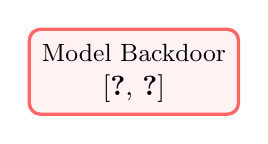
\begin{tikzpicture}[
  vuln/.style={rectangle, rounded corners, draw=red!60, fill=red!5, very thick},
  ]
 \node [vuln] (v) {
    \begin{tabular}{c}
    \makebox[2cm][c]{\small Model Backdoor} \\
    \cite{10.1016/j.infsof.2025.107707,11422005}
    \end{tabular}
 };
  \end{tikzpicture} \\
\end{tabular}
};

\node[base] (infer) [below=of tt, xshift=-3cm] {
  \begin{tabular}{cc}
  \multicolumn{2}{c}{\textbf{Inference}} \\
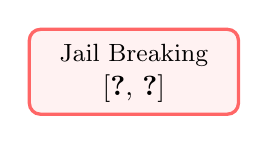
\begin{tikzpicture}[
  vuln/.style={rectangle, rounded corners, draw=red!60, fill=red!5, very thick},
  ]
 \node [vuln] (v) {
    \begin{tabular}{c}
    \makebox[2cm][c]{\small Jail Breaking} \\
    \cite{10.1007/s10515-026-00628-7,11417765}
    \end{tabular}
 };
  \end{tikzpicture} &
  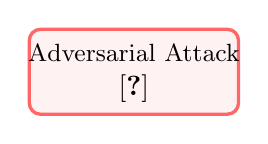
\begin{tikzpicture}[
  vuln/.style={rectangle, rounded corners, draw=red!60, fill=red!5, very thick},
  ]
 \node [vuln] (v) {
    \begin{tabular}{c}
    \makebox[2cm][c]{\small Adversarial Attack} \\
    \cite{10.1007/s10515-024-00464-7}
    \end{tabular}
 };
  \end{tikzpicture} \\
  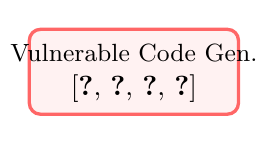
\begin{tikzpicture}[
  vuln/.style={rectangle, rounded corners, draw=red!60, fill=red!5, very thick},
  ]
 \node [vuln] (v) {
    \begin{tabular}{c}
    \makebox[2cm][c]{\small Vulnerable Code Gen.} \\
    \cite{copilotsecurity,10301242,10538871,GLAS2026104842}
    \end{tabular}
 };
  \end{tikzpicture} &
  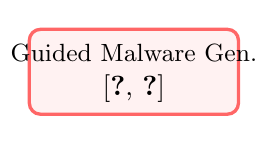
\begin{tikzpicture}[
  vuln/.style={rectangle, rounded corners, draw=red!60, fill=red!5, very thick},
  ]
 \node [vuln] (v) {
    \begin{tabular}{c}
    \makebox[2cm][c]{\small Guided Malware Gen.} \\
    \cite{ITURBE2024104077,llmbackdoordet} % improper article ID. The article leverage LLM for attacking.
    \end{tabular}
 };
  \end{tikzpicture} \\
  \multicolumn{2}{c}{
    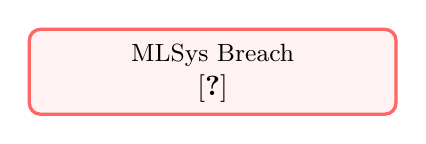
\begin{tikzpicture}[
  vuln/.style={rectangle, rounded corners, draw=red!60, fill=red!5, very thick},
  ]
 \node [vuln] (v) {
    \begin{tabular}{c}
    \makebox[4cm][c]{\small MLSys Breach} \\
    \cite{10.1145/3756681.3757083}
    \end{tabular}
 };
    \end{tikzpicture}
  } \\
\end{tabular}
};


\node[base] (harness) [right=of infer] {
  \begin{tabular}{cc}
  \multicolumn{2}{c}{\textbf{Agent Harness}} \\
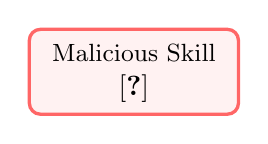
\begin{tikzpicture}[
  vuln/.style={rectangle, rounded corners, draw=red!60, fill=red!5, very thick},
  ]
 \node [vuln] (v) {
   \begin{tabular}{c}
    \makebox[2cm][c]{\small Malicious Skill} \\
    \cite{skillvulns}
   \end{tabular}
 };
  \end{tikzpicture} &
  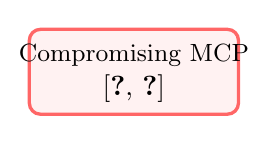
\begin{tikzpicture}[
  vuln/.style={rectangle, rounded corners, draw=red!60, fill=red!5, very thick},
  ]
 \node [vuln] (v) {
   \begin{tabular}{c}
    \makebox[2cm][c]{\small Compromising MCP} \\
    \cite{10.1145/3814959,mcpvulns}
   \end{tabular}
 };
  \end{tikzpicture} \\
  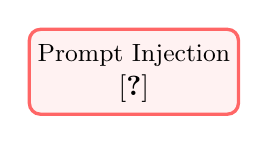
\begin{tikzpicture}[
  vuln/.style={rectangle, rounded corners, draw=red!60, fill=red!5, very thick},
  ]
 \node [vuln] (v) {
   \begin{tabular}{c}
    \makebox[2cm][c]{\small Prompt Injection} \\
    \cite{11536564}
   \end{tabular}
 };
  \end{tikzpicture} &
  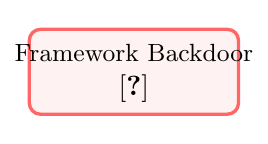
\begin{tikzpicture}[
  vuln/.style={rectangle, rounded corners, draw=red!60, fill=red!5, very thick},
  ]
 \node [vuln] (v) {
   \begin{tabular}{c}
    \makebox[2cm][c]{\small Framework Backdoor} \\
    \cite{11536564}
   \end{tabular}
 };
  \end{tikzpicture}  \\

  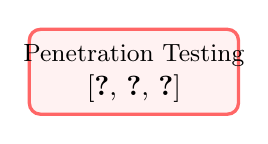
\begin{tikzpicture}[
  vuln/.style={rectangle, rounded corners, draw=red!60, fill=red!5, very thick},
  ]
 \node [vuln] (v) {
  \begin{tabular}{c}
    \makebox[2cm][c]{\small Penetration Testing} \\
    \cite{10970188,11418046,10.1145/3766895}
  \end{tabular}
 };
  \end{tikzpicture} &
  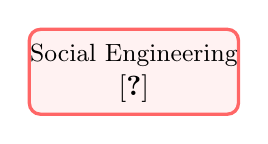
\begin{tikzpicture}[
  vuln/.style={rectangle, rounded corners, draw=red!60, fill=red!5, very thick},
  ]
 \node [vuln] (v) {
    \begin{tabular}{c}
    \makebox[2cm][c]{\small Social Engineering} \\
    \cite{10187385}
    \end{tabular}
 };
  \end{tikzpicture} 
\end{tabular}
};

\end{tikzpicture}
% \end{document}

  \caption{The vulnerabilities of an LLM in \textit{Training}, \textit{Inference},
  and \textit{Agent} stage. \\
   {\small Each citation in this figure represents an attack made by a previous research.}
  }
  \label{fig:llmrisk}
\end{figure}

\subsection{Implications of Training Stage Vulnerabilities}
In its training and fine-tuning process, Large Language Models
are susceptible to \textit{data poisoning} and \textit{backdoor injection}
attacks. Speaking of Code Language Models (CLMs), its training data
may be contaminated by malicious or vulnerable code snippets.
Consequently, in their inference stage, the generated code contains
similar patterns of vulnerability or malice; certain LLM-based
bug detector may suffer reduced effectiveness. As an increasing proportion
of code is written by CLMs, \textit{data poisoning} is capable of
polluting Software Supply Chain with problematic software packages.
For instance, M. Jahanshahi et al. made a large scale investigation
into the use of Open Source Software in LLM training, and observed
a drop in vulnerability rate when the LLM is trained with "cleaner"
code (e.g. whose CVEs are resolved) \citep{11028470}. Such observations
calls for data poisoning mitigation techniques (e.g. \citep{11344010}) to 
sanitize the defects in the training data.

% SSC attack vector 1.
\par Researchers have noticed the existence of \textit{backdoor}s in
these CLMs, which enabled the attacker to manipulate a model's response
with a trigger in the prompt to obtain malicious code from the model's
output \citep{li2021backdoorattackspretrainedmodels}. 
Y. Qu et al. conducted a review of LLM backdoor attacks, 
fine-tuning based  methods, and
applications (including deliberate malicious code injection)
\citep{10.1016/j.infsof.2025.107707}. Like \textit{data poisoning},
\textit{backdoor attack} can also inject malicious package into
Software Supply Chain.



